\documentclass[a4paper, titlepage,12pt]{article}
\usepackage[swedish,english]{babel}
\usepackage{listings}
\usepackage{verbatimbox}
\usepackage{xcolor}
\usepackage{pgfplots}
\usepackage{tikz}
\usepackage{amsmath}
\usepackage{float}
\usetikzlibrary{datavisualization}
\definecolor{codegreen}{rgb}{0,0.6,0}
\definecolor{codepurple}{rgb}{0.5,0,0.5}
\definecolor{backcolor}{rgb}{0.97,0.97,0.97}
\lstdefinestyle{mystyle}{
	commentstyle=\color{codegreen},
	keywordstyle=\color{magenta},
	numberstyle=\color{gray}\ttfamily\footnotesize,
	backgroundcolor=\color{backcolor},
	basicstyle=\ttfamily\footnotesize,
	stringstyle=\color{codepurple},
	numbers=left,
	tabsize=4
}
\lstset{style=mystyle}

\title{Computer Vision\\Assignment 3 \& 4}
\author{Adam Temmel (adte1700)}
\date{\today}

\begin{document}
\maketitle

\section*{Assignment 3}
	\subsubsection*{Mark the following points in a graph. Draw the Hough space for the points (using $\rho$ and $\theta$). In the Hough space, identify the crossing of the graphs (or the ”best possible solution”). Draw the line corresponding to the best solution in the graph.}

	I constructed the following plots (using the $\rho = x cos(\theta) + y sin(\theta)$ formula):

	\begin{figure}[h!]
		\begin{center}
		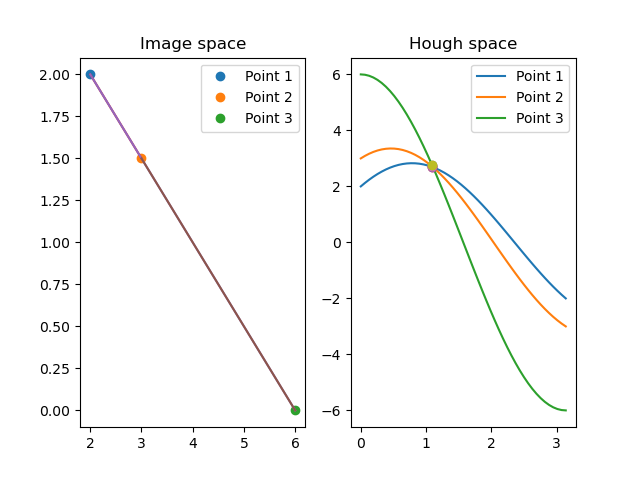
\includegraphics[scale=0.8]{./pts_1.png}
			\caption{Hough space generated from the points (2, 2), (3, 1.5), (6, 0)}
		\end{center}
	\end{figure}

	A line has been drawn between the points which crossing each other.
	\newpage

	\begin{figure}[h!]
		\begin{center}
		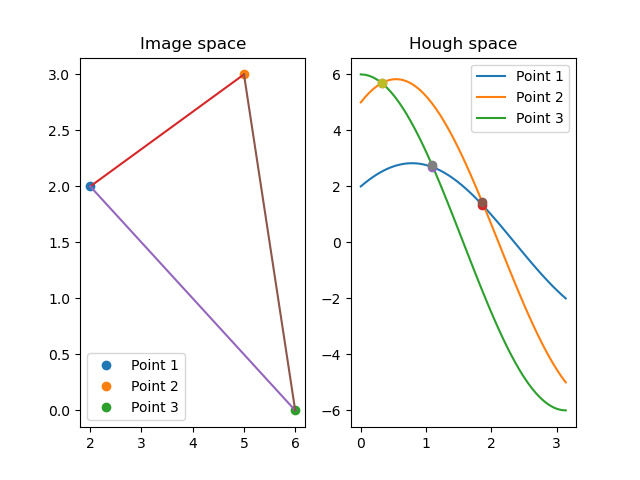
\includegraphics[scale=0.8]{./pts_2.png}
			\caption{Hough space generated from the points (2, 2), (5, 3), (6, 0)}
		\end{center}
	\end{figure}

	Here, several crossings appeared, but only once per point combination. As such, I plotted all of the crossings, as none of the available crossings seemed better or worse than the others.

\end{document}
